
\section{Tutorial}
\label{section:tutorial}
\setcounter{footnote}{0}

Here's a tutorial walk-through of how to use \rscape. This should
suffice to get you started.

\subsection {Modes of \rscape}

For an input alignment, \rscape\ reports all pairs that have
covariation scores with E-values smaller than a target E-value.\\

\noindent
The E-values are calculated in one of two ways:

\begin{tabular}{ll}
\multicolumn{2}{l}{\textbf{A one-set statistical test:} \textit{default}} \\ 
 & \\ 
\textbf{}   & E-values are calculated assuming that all pairs are possible.\\
\textbf{}   & This is the default behavior of \rscape.\\
 & \\ 
\multicolumn{2}{l}{\textbf{A two-set statistical test: } \prog{option -s}} \\ 
 & \\ 
\textbf{}   & If the alignment has associated a \emph{given structure}, \textbf{\prog{option -s}} performs two independent statistical tests: \\
\textbf{}   & one for the pairs included in the structure, a different one for all the remaining possible pairs.\\
\textbf{}   & It also draws the given consensus structure annotated with the significantly covarying base pairs.\\
 & \\ 
\end{tabular}

\subsection {Option --fold}

After performing one of the two statistical tests, this option:\\

\begin{tabular}{ll}
\textbf{}   & Builds the best consensus structure that includes the largest possible number of significantly covarying pairs,\\
\textbf{}   & \hspace{5mm}\emph{the maximum-covariation optimal consensus structure}. The algorithm identifies pseudoknots and\\
\textbf{}   & \hspace{5mm}other not nested interactions by running a cascade of nested algorithms until all covarying pairs\\
\textbf{}   & \hspace{5mm}are taken into account.\\
\textbf{}   & Draws the \emph{maximum-covariation optimal consensus structure} annotated with the significantly \\
\textbf{}   & \hspace{5mm}covarying base pairs.\\
\textbf{}   & It also returns the alignment in Stockholm format annotated with the max-cov optimal consensus structure.\\
 & \\ 
\end{tabular}


I'll show examples of running each mode, using examples in the
\ccode{tutorial/} subdirectory of the distribution.


\subsection{Files used in the tutorial}

The subdirectory \prog{/tutorial} in the \rscape\ distribution contains the
files used in the tutorial. 

The tutorial provides several examples of RNA structural
alignments, all in Stockholm format:

\begin{sreitems}{\emprog{updated\_Arisong.sto}}
\item[\emprog{updated\_Arisong.sto}] Structural alignment of the ciliate
  Arisong RNA. This alignment is an updated
  version of the one published in~\citep{JungEddy11}.
\item[\emprog{ar14.sto}] Structural alignment of the $\alpha$-proteobacteria ncRNA ar14. This alignment is an updated version of the one
  published in~\citep{delVal12}.
\item[\emprog{manA.sto}] Alignment of the manA RNA motif~\citep{Weinberg09,Weinberg10} provided in the Zasha Weinberg database (ZWD)~\citep{ZWD18}.
\item[\emprog{RF00005.sto}] Rfam v12.0~\citep{Nawrocki15} seed alignment of tRNA. 
\item[\emprog{RF00001-noss.sto}] Rfam v12.0 seed alignment of 5S rRNA, after removing the consensus secondary structure. 
\end{sreitems}


\subsection{Running \rscape\, on one alignment file}
To run \rscape\ with default parameters on alignment file
\prog{tutorial/updated\_Arisong.sto} use:\\

\user{bin/R-scape tutorial/updated\_Arisong.sto}\\

\noindent
The output is a list of the significantly covarying positions under the one-set test

\begin{sreoutput}
# R-scape :: RNA Structural Covariation Above Phylogenetic Expectation
# R-scape 1.2.0 (January 2019)
# Copyright (C) 2016-2019 Howard Hughes Medical Institute.
# Freely distributed under the GNU General Public License (GPLv3).
# - - - - - - - - - - - - - - - - - - - - - - - - - - - - - - - - - - - -
# One-set statistical test (all pairs are tested as equivalent) 
#
# MSA updated_Arisong_1 nseq 95 (95) alen 65 (150) avgid 66.35 (64.97) nbpairs 20 (20)
#
# Method Target_E-val [cov_min,conv_max] [FP | TP True Found | Sen PPV F] 
# GTp    0.05         [-9.82,121.80]     [0 | 4 20 4 | 20.00 100.00 33.33] 
#
#       left_pos       right_pos        score          E-value       substitutions      power
#-------------------------------------------------------------------------------------------------------
*	      98	     106	121.80433	3.95915e-08	44		0.44
*	     122	     137	91.75573	8.34366e-05	59		0.55
*	      96	     108	89.46430	0.000148586	25		0.26
*	     120	     139	75.03790	0.00537656	85		0.70
\end{sreoutput}
A star ``*'' in the first column indicates that the pair is part of
the annotated structure in the \prog{updated\_Arisong.sto} file. A
blank indicates a pair that is not compatible with the structure. A
``$\sim$`` indicates an interaction not in the annotated structure but
compatible with it (none in this example).

The Arisong RNA in \prog{tutorial/updated\_Arisong.sto} has a proposed
secondary structure.  Instead of testing all pairs as equivalent, we
may want to test the significance of the given structure as a one set
of pairs, and independently that of the rest of all possible pairs.
In order to do a two-set test use:\\

\user{bin/R-scape -s tutorial/updated\_Arisong.sto}\\

\noindent
The output is a list of the significantly covarying positions under the two-set test.

\begin{sreoutput}
# R-scape :: RNA Structural Covariation Above Phylogenetic Expectation
# R-scape 1.2.0 (January 2019)
# Copyright (C) 2016-2019 Howard Hughes Medical Institute.
# Freely distributed under the GNU General Public License (GPLv3).
# - - - - - - - - - - - - - - - - - - - - - - - - - - - - - - - - - - - -
# Two-set statistical test (one test for annotated basepairs, another for all other pairs)
#
# Structure obtained from the msa
# SS_cons ::::::::::::::::::::::::::::::::::::::::::::::::::::::::::::
#
# SS_cons :::::::::::::::::::::::::::::::::<<<<<<<___>>>>>>><<<<<<--<<
#
# SS_cons <<<<<_______>>>->>>>-->>>>>>::
#
# left_pos      right_pos    substitutions      power
#--------------------------------------------------------
# 94		110		34		0.35
# 95		109		29		0.30
# 96		108		25		0.26
# 97		107		58		0.55
# 98		106		44		0.44
# 99		105		15		0.14
# 100		104		20		0.20
# 111		148		0		0.00
# 112		147		18		0.18
# 113		146		1		0.00
# 114		145		9		0.07
# 115		144		48		0.47
# 116		143		110		0.80
# 119		140		88		0.72
# 120		139		85		0.70
# 121		138		97		0.76
# 122		137		59		0.55
# 123		135		73		0.64
# 124		134		27		0.28
# 125		133		31		0.32
#
# BPAIRS 20
# avg substitutions per BP  43.5
# BPAIRS expected to covary 7.7
# BPAIRS observed to covary 12
#
#
# Method Target_E-val [cov_min,cov_max] [FP | TP True Found | Sen PPV F] 
# GTp    0.05         [-9.82,121.80]     [0 | 12 20 12 | 60.00 100.00 75.00] 
#
#       left_pos       right_pos        score          E-value       substitutions      power
#-------------------------------------------------------------------------------------------------------
*	      98	     106	121.80433	3.80688e-10	44		0.44
*	     122	     137	91.75573	8.02275e-07	59		0.55
*	      96	     108	89.46430	1.42871e-06	25		0.26
*	     120	     139	75.03790	5.16977e-05	85		0.70
*	     119	     140	58.25176	0.00255411	88		0.72
*	     121	     138	57.96915	0.00265136	97		0.76
*	      94	     110	56.91065	0.00330664	34		0.35
*	     124	     134	55.84207	0.00409643	27		0.28
*	     123	     135	55.50367	0.00439184	73		0.64
*	      99	     105	53.86423	0.00611505	15		0.14
*	      97	     107	44.72409	0.0293269	58		0.55
*	     115	     144	41.87792	0.0490385	48		0.47
\end{sreoutput}
The scores of the pairs are identical to those in the one-set
test. The E-values have changed relative to those of the one-set test.


\subsection{The --fold option}

\user{bin/R-scape --fold tutorial/updated\_Arisong.sto}\\

\noindent
The output includes first the same output as default \rscape\ alone,
followed by \rscape's proposed structure that under the heading ``\#
The predicted structure'' as follows,

\begin{sreoutput}
# R-scape :: RNA Structural Covariation Above Phylogenetic Expectation
# R-scape 1.2.0 (January 2019)
# Copyright (C) 2016 Howard Hughes Medical Institute.
# Freely distributed under the GNU General Public License (GPLv3).
#-------------------------------------------------------------------------------------------------------
# MSA updated_Arisong_1 nseq 95 (95) alen 65 (150) avgid 66.35 (64.97) nbpairs 20 (20)
# One-set statistical test (all pairs are tested as equivalent) 
#
#
# Method Target_E-val [cov_min,cov_max] [FP | TP True Found | Sen PPV F] 
# GTp    0.05         [-9.82,121.80]     [0 | 4 20 4 | 20.00 100.00 33.33] 
#
#       left_pos       right_pos        score          E-value       substitutions      power
#-------------------------------------------------------------------------------------------------------
*	      98	     106	121.80433	3.95915e-08	44		0.47
*	     122	     137	91.75573	8.34366e-05	59		0.60
*	      96	     108	89.46430	0.000148586	25		0.27
*	     120	     139	75.03790	0.00537656	85		0.75

# The predicted structure
# SS_cons ::::::::::::::::::::::::::::::::::::::::::::::::::::::::::::
#
# SS_cons ::::::::::::::::::::::::::::::::::<<<<<_____>>>>>:<<<<<---<<
#
# SS_cons <<<<<_______>>>->>>>--->>>>>::
#
# left_pos      right_pos    substitutions      power
#--------------------------------------------------------
# 95		109		29		0.32
# 96		108		25		0.27
# 97		107		58		0.59
# 98		106		44		0.47
# 99		105		15		0.14
# 111		148		0		0.00
# 112		147		18		0.18
# 113		146		1		0.00
# 114		145		9		0.06
# 115		144		48		0.51
# 119		140		88		0.77
# 120		139		85		0.75
# 121		138		97		0.81
# 122		137		59		0.60
# 123		135		73		0.69
# 124		134		27		0.30
# 125		133		31		0.34
#
# BPAIRS 17
# avg substitutions per BP  41.6
# BPAIRS expected to covary 6.8
# BPAIRS observed to covary 4
#
#
# Method Target_E-val [cov_min,cov_max] [FP | TP True Found | Sen PPV F] 
# GTp    0.05         [-9.82,121.80]     [0 | 4 17 4 | 23.53 100.00 38.10] 
#
# in_cyk in_given   left_pos       right_pos      score           E-value    substitutions      power
#----------------------------------------------------------------------------------------------------------------
*	*	        98	       106	121.80433	3.95915e-08	44		0.47
*	*	       122	       137	91.75573	8.34366e-05	59		0.60
*	*	        96	       108	89.46430	0.000148586	25		0.27
*	*	       120	       139	75.03790	0.00537656	85		0.75
\end{sreoutput}

The structure predicted by \rscape\ includes all the basepairs
reported as covarying, provided that those can be arranged into one
single structure (including pseudoknots and other non Watson-Crick
interactions). The \rscape\ folding algorithm cannot deal with
residues that covary with more than one other residue, such as is the case for
alternative structures or triplets.

\noindent
Similarly using

\user{bin/R-scape -s --fold tutorial/updated\_Arisong.sto}\\

\noindent
The output includes first the same output as \emprog{option -s} of
\rscape\ alone, followed by \rscape's proposed structure including a
maximal number of the covariations obtained under the two-set test.


\begin{sreoutput}
# R-scape :: RNA Structural Covariation Above Phylogenetic Expectation
# R-scape 1.2.0 (January 2019)
# Copyright (C) 2016 Howard Hughes Medical Institute.
# Freely distributed under the GNU General Public License (GPLv3).
#-------------------------------------------------------------------------------------------------------
# MSA updated_Arisong_1 nseq 95 (95) alen 65 (150) avgid 66.35 (64.97) nbpairs 20 (20)
# Two-set statistical test (one test for annotated basepairs, another for all other pairs)
#
# Structure obtained from the msa
# SS_cons ::::::::::::::::::::::::::::::::::::::::::::::::::::::::::::
#
# SS_cons :::::::::::::::::::::::::::::::::<<<<<<<___>>>>>>><<<<<<--<<
#
# SS_cons <<<<<_______>>>->>>>-->>>>>>::
#
# left_pos      right_pos    substitutions      power
#--------------------------------------------------------
# 94		110		34		0.37
# 95		109		29		0.32
# 96		108		25		0.27
# 97		107		58		0.59
# 98		106		44		0.47
# 99		105		15		0.14
# 100		104		20		0.21
# 111		148		0		0.00
# 112		147		18		0.18
# 113		146		1		0.00
# 114		145		9		0.06
# 115		144		48		0.51
# 116		143		110		0.86
# 119		140		88		0.77
# 120		139		85		0.75
# 121		138		97		0.81
# 122		137		59		0.60
# 123		135		73		0.69
# 124		134		27		0.30
# 125		133		31		0.34
#
# BPAIRS 20
# avg substitutions per BP  43.5
# BPAIRS expected to covary 8.2
# BPAIRS observed to covary 12
#
#
# Method Target_E-val [cov_min,cov_max] [FP | TP True Found | Sen PPV F] 
# GTp    0.05         [-9.82,121.80]     [0 | 12 20 12 | 60.00 100.00 75.00] 
#
#       left_pos       right_pos        score          E-value       substitutions      power
#-------------------------------------------------------------------------------------------------------
*	      98	     106	121.80433	3.80688e-10	44		0.47
*	     122	     137	91.75573	8.02275e-07	59		0.60
*	      96	     108	89.46430	1.42871e-06	25		0.27
*	     120	     139	75.03790	5.16977e-05	85		0.75
*	     119	     140	58.25176	0.00255411	88		0.77
*	     121	     138	57.96915	0.00265136	97		0.81
*	      94	     110	56.91065	0.00330664	34		0.37
*	     124	     134	55.84207	0.00409643	27		0.30
*	     123	     135	55.50367	0.00439184	73		0.69
*	      99	     105	53.86423	0.00611505	15		0.14
*	      97	     107	44.72409	0.0293269	58		0.59
*	     115	     144	41.87792	0.0490385	48		0.51

# The predicted structure
# SS_cons ::::::::::::::::::::::::::::::::::::::::::::::::::::::::::::
#
# SS_cons :::::::::::::::::::::::::::::::::<<<<<<_____>>>>>><<<<<---<<
#
# SS_cons <<<<<_______>>>->>>>--->>>>>::
#
# left_pos      right_pos    substitutions      power
#--------------------------------------------------------
# 94		110		34		0.37
# 95		109		29		0.32
# 96		108		25		0.27
# 97		107		58		0.59
# 98		106		44		0.47
# 99		105		15		0.14
# 111		148		0		0.00
# 112		147		18		0.18
# 113		146		1		0.00
# 114		145		9		0.06
# 115		144		48		0.51
# 119		140		88		0.77
# 120		139		85		0.75
# 121		138		97		0.81
# 122		137		59		0.60
# 123		135		73		0.69
# 124		134		27		0.30
# 125		133		31		0.34
#
# BPAIRS 18
# avg substitutions per BP  41.2
# BPAIRS expected to covary 7.2
# BPAIRS observed to covary 12
#
#
# Method Target_E-val [cov_min,cov_max] [FP | TP True Found | Sen PPV F] 
# GTp    0.05         [-9.82,121.80]     [0 | 12 18 12 | 66.67 100.00 80.00] 
#
# in_cyk in_given   left_pos       right_pos      score           E-value    substitutions      power
#----------------------------------------------------------------------------------------------------------------
*	*	        98	       106	121.80433	3.80688e-10	44		0.47
*	*	       122	       137	91.75573	8.02275e-07	59		0.60
*	*	        96	       108	89.46430	1.42871e-06	25		0.27
*	*	       120	       139	75.03790	5.16977e-05	85		0.75
*	*	       119	       140	58.25176	0.00255411	88		0.77
*	*	       121	       138	57.96915	0.00265136	97		0.81
*	*	        94	       110	56.91065	0.00330664	34		0.37
*	*	       124	       134	55.84207	0.00409643	27		0.30
*	*	       123	       135	55.50367	0.00439184	73		0.69
*	*	        99	       105	53.86423	0.00611505	15		0.14
*	*	        97	       107	44.72409	0.0293269	58		0.59
*	*	       115	       144	41.87792	0.0490385	48		0.51
\end{sreoutput}


\subsection{Example of an RNA with pseudoknots}

After version 1.2.0, \rscape\ annotates pseudoknots. \rscape's folding
algorithm is capable of predicting pseudoknots using a cascade of
dynamic programming algorithms.  In addition, if the structure given
with the input alignment includes pseudoknots, \rscape\ uses the
program R2R to automatically include the pseudoknots in the display of
the consensus structure.

Consider the manA RNA motif. Both the proposed structure for manA RNA
and the predicted \rscape\ structure have 2 pseudoknots with
covariation support:

\user{bin/R-scape -s --fold tutorial/manA.sto}\\


\begin{sreoutput}
# R-scape :: RNA Structural Covariation Above Phylogenetic Expectation
# R-scape 1.2.0 (January 2019)
# Copyright (C) 2016-2019 Howard Hughes Medical Institute.
# Freely distributed under the GNU General Public License (GPLv3).
#-------------------------------------------------------------------------------------------------------
# MSA manA nseq 193 (193) alen 189 (350) avgid 74.06 (71.38) nbpairs 62 (93)
# Two-set statistical test (one test for annotated basepairs, another for all other pairs)
#
# Structure obtained from the msa
# SS_cons   <<<<<_________________________________>>>>>:::::[[[[[,,,<<--
# SS_cons_1 ::::::::::::::::::::::::::::::::::::::::::::::::::::::::::::
# SS_cons_2 ::::::::::::::::::::::::::::::::::::::::::::::::::::::::::::
#
# SS_cons   -----------<<<<<<__________________>>>>>>---->>,,,,((-((((,,
# SS_cons_1 ::::::::::::::::::::::::::::::::::::::::::::::::::::::::::::
# SS_cons_2 ::::::::::::::::::::::::::::::::::::::::::::::::::::::::::::
#
# SS_cons   ,,,,,,,,,,,,,,,,,,,,,,,,,,,,,<<<_______>>>,<<<<<<___________
# SS_cons_1 ::::::::::::::::::::::::::::::::::<<<<______________________
# SS_cons_2 ::::::::::::::::::::::::::::::::::::::::::::::::::::::::::::
#
# SS_cons   ____________________>>>>>>,,,<<<<<____________>>>>>,,))))--)
# SS_cons_1 _______________________________________>>>>:::::::::::::::::
# SS_cons_2 ::::::::::::::::::::::::::::::::::::::::::::::::::::::::::::
#
# SS_cons   ),,,,<<<<<<<------------<<<<____________________________>>>>
# SS_cons_1 ::::::::::::::::::::::::::::::::::::::::::::::::::::::::::::
# SS_cons_2 :::::::::::::::::::::::::::::::::<<<-<______________________
#
# SS_cons   ------->>>>>>>,,<<<<<_____________>>>>>]]]]]::::::
# SS_cons_1 ::::::::::::::::::::::::::::::::::::::::::::::::::
# SS_cons_2 _________________________>>>>:::::::::::::::::::::
#

  ...

  ...
  
# The predicted structure
# SS_cons   <<<<<_________________________________>>>>>:[---[[[[[,,,<<--
# SS_cons_1 ::::::::::::::::::::::::::::::::::::::::::::::::::::::::::::
# SS_cons_2 ::::::::::::::::::::::::::::::::::::::::::::::::::::::::::::
#
# SS_cons   -----------<<<<<<__________________>>>>>>---->>,(--((-((((,,
# SS_cons_1 ::::::::::::::::::::::::::::::::::::::::::::::::::::::::::::
# SS_cons_2 ::::::::::::::::::::::::::::::::::::::::::::::::::::::::::::
#
# SS_cons   ,,,,,,,,,,,,,,,,,,,,,,,,,,,,,<<<_______>>>,<<<<<<___________
# SS_cons_1 ::::::::::::::::::::::::::::::::::<<<<______________________
# SS_cons_2 ::::::::::::::::::::::::::::::::::::::::::::::::::::::::::::
#
# SS_cons   ____________________>>>>>>,,,<<<<<---<____>--->>>>>,,))))--)
# SS_cons_1 _______________________________________>>>>:::::::::::::::::
# SS_cons_2 ::::::::::::::::::::::::::::::::::::::::::::::::::::::::::::
#
# SS_cons   )--),<<<<<<<------------<<<<____________________________>>>>
# SS_cons_1 ::::::::::::::::::::::::::::::::::::::::::::::::::::::::::::
# SS_cons_2 :::::::::::::::::::::::::::::::::<<<-<<_____________________
#
# SS_cons   ------->>>>>>>,,<<<<<_____________>>>>>]]]]]-]::::
# SS_cons_1 ::::::::::::::::::::::::::::::::::::::::::::::::::
# SS_cons_2 _______________________>->>>>:::::::::::::::::::::
#
\end{sreoutput}

\noindent
 The ``SS\_cons\_1'' and ``SS\_cons\_2'' lines describe the
 interactions that are not nested relative to the main ``SS\_cons''
 structure.

\rscape\, uses R2R to produce figures of the consensus structures
where pseudoknots are also annotated.  \rscape] option -s produces the
  file \emprog{tutorial/manA.R2R.sto.\{pdf,svg\}} with the structure
  annotated in the input alignment. \rscape] option --fold produces the
    file \emprog{tutorial/manA.fold.R2R.sto.\{pdf,svg\}} with the
    structure produced by \rscape. See Figure~\ref{fig:manA_r2r}.


 \begin{figure}[h]
   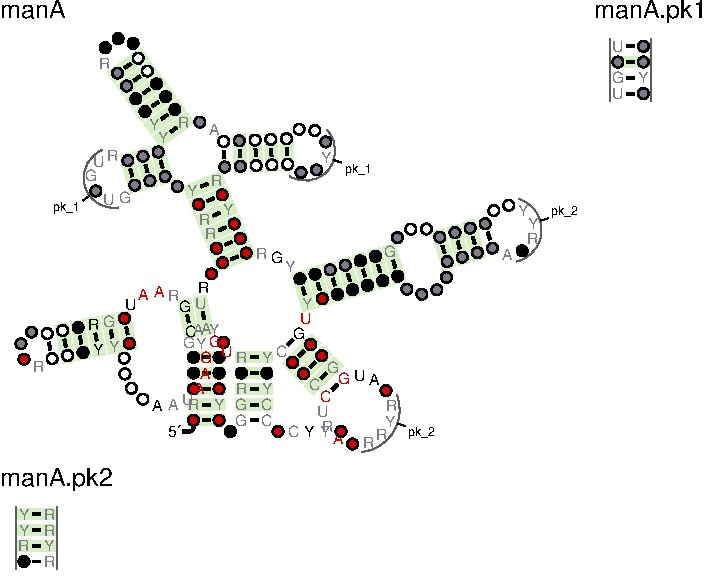
\includegraphics[scale=0.7]{manA_R2R.pdf} 
  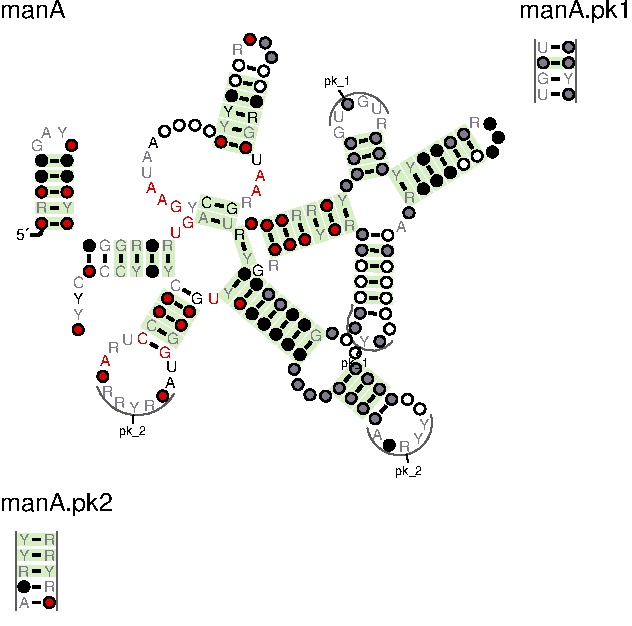
\includegraphics[scale=0.7]{manA_fold_R2R.pdf} 
  \caption{\small\textbf{Left:}
    \emprog{tutorial/manA.R2R.sto.\{pdf,svg\}}, the consensus
    secondary structure given in the input alignment, depicted by
    \rscape, using the program R2R.  \textbf{Right:}
    \emprog{tutorial/manA.fold.R2R.sto.\{pdf,svg\}}, The consensus
    structure produced by \rscape\ (option --fold).  Base pairs with
    covariation scores equal or below the target E-value (0.05 as
    default) are depicted in green.  }
 \label{fig:manA_r2r}
 \end{figure}
 

 \subsection{Single sequence structure prediction}

 If the alignment includes only one sequence, no statistical test is performed. \\

 \noindent
 \user{bin/R-scape --fold tutorial/manA-oneseq.sto}\\
%
 reports the best structure given the sequence. No covariation support
 is possible for any of the basepairs reported from this
 analysis. Structures produced this way have to taken with great
 skepticism. 

 \subsection{Default parameters}

Default parameters are:

\begin{sreitems}{\emprog{Pairwise percent identity:}}
\item[\emprog{Target E-value:}]default is 0.05. \rscape\, reports
  pairs which covariation score has E-value smaller or equal to the
  target value.  The target E-value can be changed with option
  \emprog{-E <x>}, $x >= 0$.

\item[\emprog{Sequence weighting:}]Sequences are weighted according to
  the Gerstein/Sonnhammer/Chothia (GSC)
  algorithm~\citep{Gerstein94}. This algorithm is time consuming. For
  alignments with more than 1000 sequences, we use the faster
  position-based weighting algorithm~\citep{Henikoff94b}. Both
  weighting algorithms are implemented as part of the easel library.

\item[\emprog{Gaps in columns:}]Columns with more than 50\% gaps are
  removed. The gap threshold for removing columns can be modified
   using option \emprog{--gapthresh <x>} , $0<x<=1$.

 \item[\emprog{Covariation statistic:}]The default covariation statistic
   is the average product corrected G-Test (equivalent to option
   \emprog{--GTp}).

 \item[\emprog{Covariation Class:}]\rscape\ uses the 16 component
   covariation statistic (C16), unless the number of sequences in the
   alignment is $\leq$ 8 or the length of the alignment is $\leq$ 50,
   in which case it uses the two-class covariation statistic (C2). A
   particular covariation class can be selected using either
   \emprog{--C16} or \emprog{--C2}.

   The threshold for the minimum number of sequences can be changed
   with option \prog{--nseqthresh <n>}.  The threshold for the minimum
   alignment length can be changed with option \prog{--alenthresh <n>}.

 \item[\emprog{Null alignments:}]In order to estimate E-values,
   \rscape\ produces 20 null alignments, unless the product of the
   number of sequences by the length of the alignment $<$ 10,000 in
   which case the number of null alignments is 50; or $<$ 1,000 in
   which case it is 100. The number of null alignments can be
   controlled with option \emprog{--nshuffle <n>}.
 \end{sreitems}

 A full list of the \rscape\ options is found by using

 \user{\rscape\ -h}

 
 
